%%%%%%%%%%%%%%%%%%%%%%%%%%%%%%%%%%%%%%%%%%%%%%%%%%%%%%%%%%%%%%%%%%%%%%%%%%%%
% Statistics for Data Science (DataSci w203)
% Unit 4 part 1 homework
%%%%%%%%%%%%%%%%%%%%%%%%%%%%%%%%%%%%%%%%%%%%%%%%%%%%%%%%%%%%%%%%%%%%%%%%%%%%

% Setup
\documentclass[12pt,a4paper]{article}
\usepackage[inner=1.5cm,outer=1.5cm,top=2.5cm,bottom=2.5cm]{geometry}
\usepackage{graphicx, subfig}
\usepackage[english]{babel}
\usepackage{amsmath}
\usepackage{amssymb}
\numberwithin{equation}{subsection}
\usepackage{hyperref}
\usepackage{listings}


\usepackage{Sweave}
\begin{document}
\Sconcordance{concordance:Kevin_Hartman_unit_4_part_1_hw.tex:Kevin_Hartman_unit_4_part_1_hw.Rnw:%
1 54 1 2 5 169 1}

\Sconcordance{concordance:Kevin_Hartman_unit_4_part_1_hw.tex:Kevin_Hartman_unit_4_part_1_hw.Rnw:%
1 54 1 2 5 169 1}


\author{Kevin Hartman (W203 Wednesday 6:30pm Summer 2019)}
\date{5/29/2019}
\title{Statistics for Data Science \\
       Unit 4 Part 1 Homework: Discrete Random Variables}
\maketitle


%----------------------------------------------------------------------------------------
%----------------------------------------------------------------------------------------
\begin{enumerate}

\item \textbf{Best Game in the Casino}߆

You flip a fair coin 3 times, and get a different amount of money depending on how many heads you get. For 0 heads, you get \$0. For 1 head, you get \$2. For 2 heads, you get \$4. Your expected winnings from the game are \$6. 
\\
\\
\textbf{\underline{Givens:}}
\\
X is a binomial random variable based on $n$ trials with success probability $p$.

When X=x, let x be the number of heads among the $n=3$ trials with the probability of a head in each trial being $p=\frac{1}{2}$.

$$b(x;n,p) = \begin{cases}
(^n_k)p^x(1-p)^{n-x}, &x \in \{0,1,2,3,...\}\\
0, &otherwise.\\
\end{cases}
$$

$$\text{Probablity of 0 Heads: }P(X=0)=b(0;3,\frac{1}{2}) = (^3_0)(\frac{1}{2})^3 = \frac{1}{8}$$
$$\text{Probablity of 1 Heads: }P(X=1)=b(1;3,\frac{1}{2}) = (^3_1)(\frac{1}{2})^3 = \frac{3}{8}$$
$$\text{Probablity of 2 Heads: }P(X=2)=b(2;3,\frac{1}{2}) = (^3_2)(\frac{1}{2})^3 = \frac{3}{8}$$
$$\text{Probablity of 3 Heads: }P(X=3)=b(3;3,\frac{1}{2}) = (^3_3)(\frac{1}{2})^3 = \frac{1}{8}$$

	

\begin{minipage}{\linewidth}
  \centering
  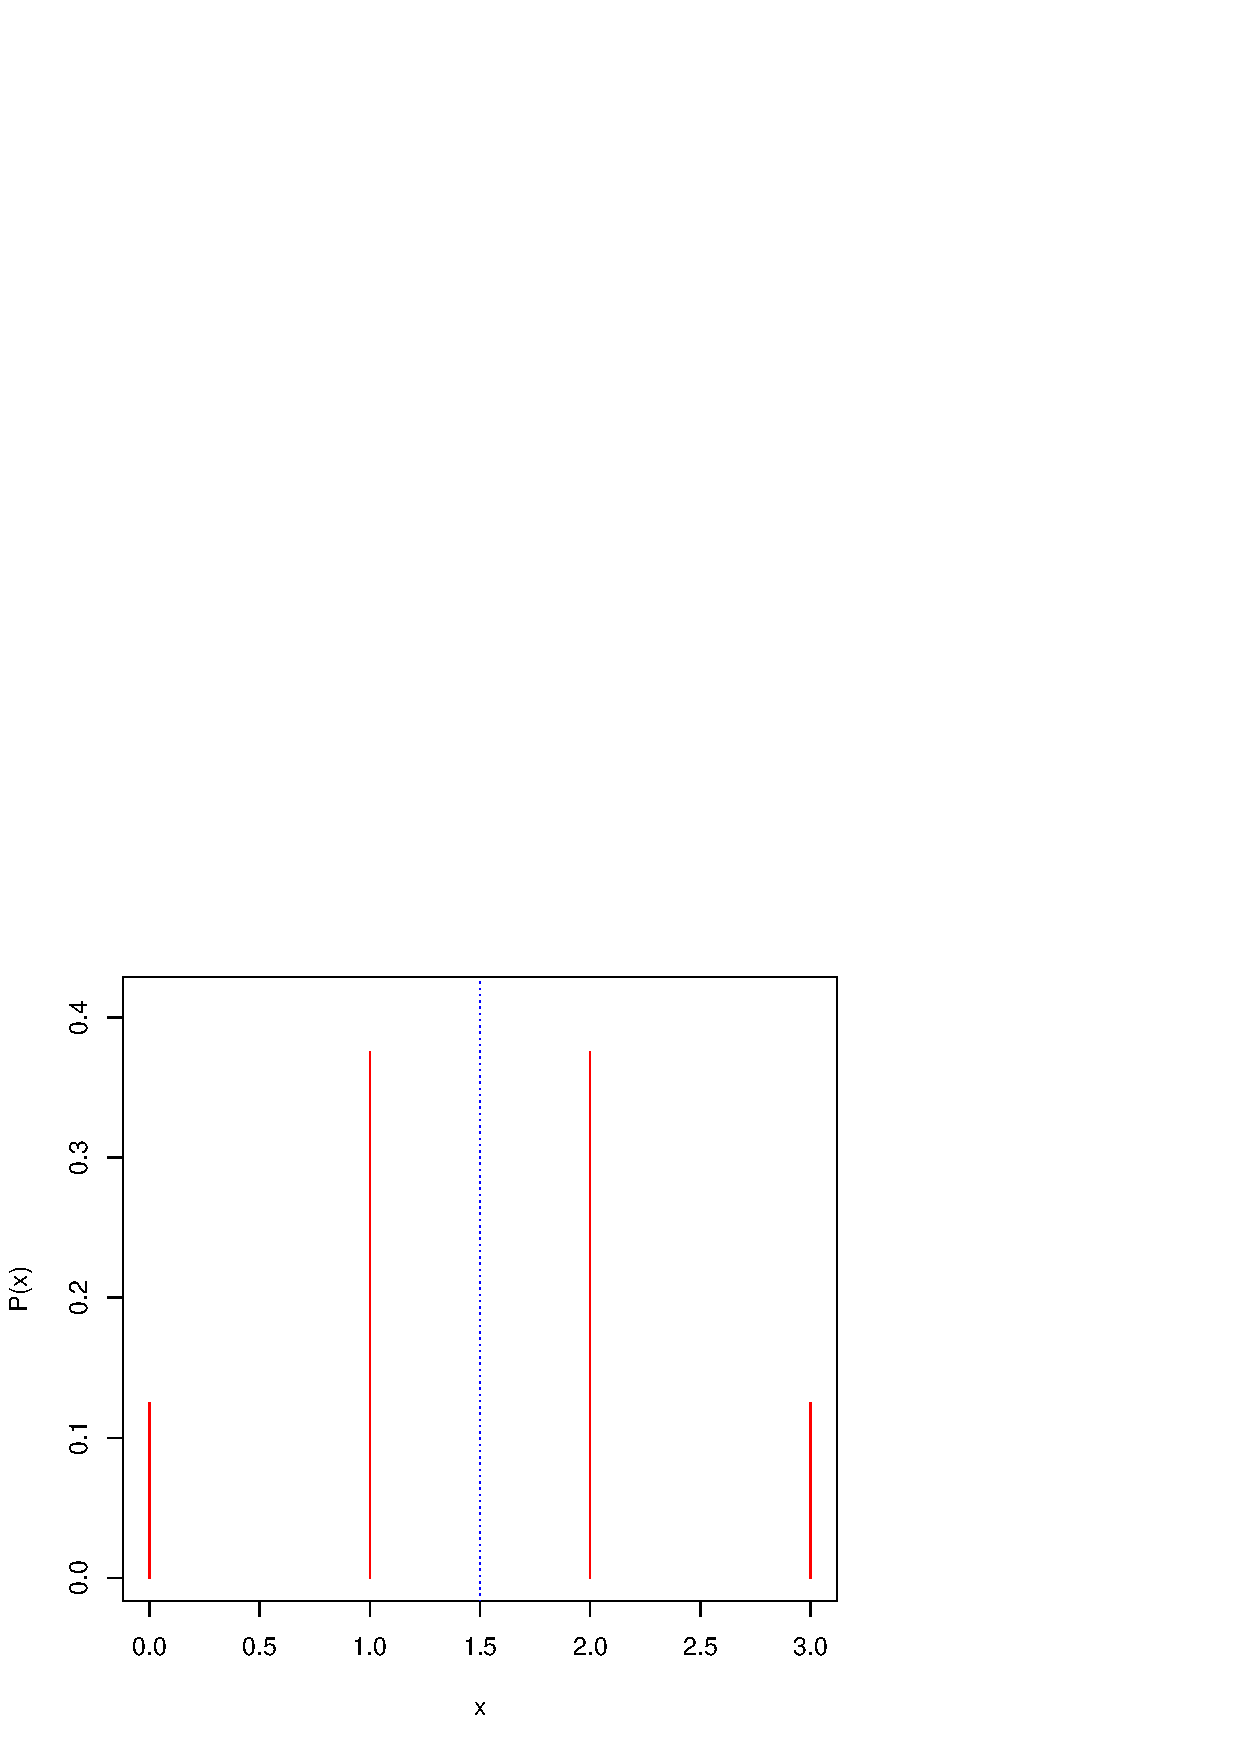
\includegraphics[width=6cm]{Kevin_Hartman_unit_4_part_1_hw-xbinom}
  \captionof{figure}{Plot of binomial distribution of n=3, p=$\frac{1}{2}$}
\end{minipage}

\begin{enumerate}
\item How much do you get paid if the coin comes up heads 3 times?
\\
\\
\textbf{\underline{Answer:}}
\\
$\text{Given fair coins, the expectation of X, } E(X) = np = 3 \cdot \frac{1}{2} = \frac{3}{2} \text{ (also shown in graph above)}$
\\
\\
The expected winnings from the game is \$6, such that $g(E(X)) = 6$
\\
\\
We also have:
\\
\\
$G(X=0) = 0$

$G(X=1) = 2$

$G(X=2) = 4$

$G(X=3) = A$
\\
\\
Using the expectation that $E(g(X)) = g(E(X))$ we can solve for A:

$$E(g(X)) = \sum_{y=0}^x g(y) \cdot p(y) = 6$$

$$(0 \cdot \frac{1}{8}) + (2 \cdot \frac{3}{8}) + (4 \cdot \frac{3}{8}) +  (A \cdot \frac{1}{8} ) = 6$$

$$(\frac{6}{8}) + (\frac{12}{8}) + (\frac{A}{8}) = 6$$

$$6 + 12 + A = 48$$

$$A = 30$$


\item Write down a complete expression for the cumulative probability function for your winnings from the game.
\\
\\
\textbf{\underline{Answer:}}
\\
%%$$\text{With} \enskip g(y) = \left\{\begin{array}{{lcl}} 0 &;& y < 1 \\  \frac{16}{3} &;& 1 \leq y < 3 \\  208 &;& y \leq 3 \end{array} \right.,\enskip  p=\frac{1}{2}, \enskip \text{and } n=3$$
%%$$\text{Winnings } = g(P(X \leq x)) = \sum_{y=0}^x g(y) \cdot \left(^n_y \right)p^y(1-p)^{n-y}$$
The cumulative probability function for the winnings, $F(g(X))$, is:
\\
\\
$F(g(X)) = \begin{cases}
0, &g(X) < 0 \\
1/8,  &0 \leq g(X) < 2 \\
1/2, &2 \leq g(X) < 4 \\
7/8, &4 \leq g(X) < 30 \\
1, &g(X) \geq 30\\
\end{cases}$

\end{enumerate}

\item \textbf{Reciprocal Dice}

Let $X$ be a random variable representing the outcome of rolling a 6-sided die.  Before the die is rolled, you are given two options:

\begin{enumerate}
\item You get $1/E(X)$ in dollars right away.
\\
\\
\textbf{\underline{Proof:}}
\\
Since each die roll has uniform probability we can compute $E(X)$ as:
\\
$$E(X) = \frac{1}{k}{\sum_j x_j} = \frac{1+2+3+4+5+6}{6} = 3.5$$
\\
\\
$1/E(X)$ is approx .28571 dollars

\item You wait until the die is rolled, then get $1/X$ in dollars.
\\
\\
\textbf{\underline{Proof:}}
\\
$\text{Given } g(X) = 1/X \text{ and } E(g(X)) = \sum_x g(x) \cdot p(x)$
\\
$$E(g(X)) = (1 \cdot \frac{1}{6}) + (\frac{1}{2} \cdot \frac{1}{6}) + (\frac{1}{3} \cdot \frac{1}{6}) + (\frac{1}{4} \cdot \frac{1}{6}) + (\frac{1}{5} \cdot \frac{1}{6}) + (\frac{1}{6} \cdot \frac{1}{6})$$
\\
$E(g(X))$ is approx .408333 dollars

\item Which option is better for you, in expectation?
\\
\\
\textbf{\underline{Answer:}}
\\
$.408333$ is greater than $.28571$. The second option is better in expectation.

\end{enumerate}

\item \textbf{The Baseline for Measuring Deviations}

Given any random variable $X$ and a real number $t$, we can define another random variable $Y = (X - t)^2$. In other words, for any random variable $X$, we can choose a real number, $t$, as a baseline and calculate the squared deviation of $X$ away from $t$.

You might wonder why we often square deviations (instead of taking an absolute value, or cubing them, etc.).  This exercise will shed some light on why this is a natural choice.

\begin{enumerate}
\item Write down an expression for $E(Y)$ and simplify it as much as you can.  Even though we haven't proved this yet, you can use the fact that for any two random variables, $A$ and $B$, $E(A + B) = E(A) + E(B)$.
\\
\textbf{\underline{Answer:}}
$$E(Y) = E[(X - t)^2] = E[(X^2 -2tX + t^2)]$$
$$= E[(X^2)] + E[(-2tX)] + E[(t^2)]$$
$$= E(X^2) - 2tE(X) + t^2$$
\item Taking a partial derivative with respect to $t$, compute the value of $t$ that minimizes $E(Y)$.  (Hint: Your answer should be a very familiar value)
\\
\newpage
\textbf{\underline{Answer:}}
$$E(Y)'_{(x, t)} = \frac{\partial }{\partial t} [E(X^2) - 2tE(X) + t^2]$$
$$= - 2E(X) + 2t$$
$E(Y)$ approaches minimum when
$$t = E(X)$$
\item What is the value of $E(Y)$ for this choice of $t$?
(Hint: this should also be a very familiar value)
\\
\textbf{\underline{Answer:}}
\\
Replacing $t$ with $E(X)$ in $E(Y) = E(X^2) - 2tE(X) + t^2$:
$$E(X^2) - 2tE(X) + t^2 = E(X^2) - 2E(X)E(X) + [E(X)]^2$$
$$ = E(X^2) - 2[E(X)]^2 + [E(X)]^2$$
The value of $E(Y)$ at the minimum will be 
$$E(Y) = E(X^2) - [E(X)]^2$$

\end{enumerate}

\item \textbf{Optional Advanced Exercise: Heavy Tails}

One reason to study the mathematical foundation of statistics is to recognize situations where common intuition can break down.  An unusual class of distributions are those we call \textit{heavy-tailed}.  The exact definition varies, but we'll say that a heavy-tailed distribution is one for which not all moments are finite.  Consider a random variable $M$ with the following pmf:

$$p_M(x) = \begin{cases}
c/x^3, &x \in \{1,2,3,...\}\\
0, &otherwise.\\
\end{cases}
$$

where $c$ is a constant (you can calculate its value if you like, but it's not important).

\begin{enumerate}
\item Is $E(M)$ finite?
\\
\textbf{\underline{Answer:}}
\\
Yes it is finite because although this an infinite series, the sum of $c/x^3$ from 1 to $\infty$ will eventually converge.  It converges because the equation represents a p-series $(1/n^p)$ and a p-series converges when p > 1 and diverges when 0 < p < 1.

\item Is $V(M)$ finite?
\\
\textbf{\underline{Answer:}}
\\
Also finite for the same reason as (a). For $V(M)$ to be calculated the infinite series must converge.

\end{enumerate}

Heavy-tailed distributions may seem odd, but they're not as rare as you might suspect.  Researchers argue that the distribution of wealth is heavy-tailed; so is the distribution of computer file sizes, insurance payouts, and area burned by forest fires.  These random variables are problematic in that a lot of common statistical techniques don't work on them.  For this class, we'll assume that all of our variables don't have heavy-tails.

\end{enumerate}

\end{document}
